%% Where a Test Oracle Reads From
%% Evidential independence as a design criterion for differential testing
%%
%% TARGET: ISSTA (acmart/sigconf). The class is deliberate: ICSE uses the same
%% class, and the ISSTA-collocated workshops use it in a shorter format, so
%% moving DOWN (workshop) or SIDEWAYS (ICSE) is a format switch, not a rewrite.
%% Written to the full-paper shape on purpose — lowering is cheap, raising is not.
%%
%% BUILD: needs acmart.cls (texlive-publishers, or Overleaf). Not installed in
%% the development container; compile on Overleaf or a TeX Live host.

%% ---------------------------------------------------------------------------
%% SUBMISSION SWITCHES — the numbers in the margin are NOT A WORD COUNT, they are line numbers.
%% Source: acmart.cls:2516, `\if@ACM@review` -> `\ACM@mk@linecount`. I.e. what ACM's
%% own class DELIBERATELY prints in review mode, so that a reviewer can cite a line.
%% Measured: review on 9 pages, off 9 pages -- it does not change the pagination.
%%
%%   review     -> line numbers + folio. Wanted in a double-blind submission; check the CFP.
%%   anonymous  -> makes the authors "Anonymous Author(s)". Required for double-blind.
%%
%% In CAMERA-READY both are REMOVED and these are added:
%%   \acmConference[ACRONYM '27]{...}{date}{venue}
%%   \acmBooktitle{...}  \acmDOI{...}  \acmISBN{...}  \copyrightyear{...}
%% The "Conference'17, July 2017, Washington, DC, USA" at the bottom of the page is the
%% PLACEHOLDER acmart prints in the absence of \acmConference; it must also be filled at submission.
%%
%% Measured structure: body pp.1-7, Appendix A starts on p.8, REFERENCES on p.9.
%% ---------------------------------------------------------------------------
\documentclass[sigconf,review,anonymous]{acmart}

%% Fig.1 (the 2x2) is TikZ; acmart does not load it.
\usepackage{tikz}
%% Float fractions loosened so a top float is not stranded alone on a final page.
%% (Appendix B's table was also made single-column for the same reason: a table*
%% met mid-page can only go to the NEXT page top.)
\renewcommand{\dbltopfraction}{0.92}
\renewcommand{\dblfloatpagefraction}{0.85}
\renewcommand{\topfraction}{0.9}
\renewcommand{\textfraction}{0.07}

%% PAGE BUDGET — deliberately left as a parameter rather than a number.
%% ACM/ISSTA limits change per edition; fill from the current CFP, do not
%% guess. The decision that matters is not the limit but the CAP below.
%%
%% THE CAP, and it is the point of this file:
%%   Sec.5 (case study) MUST NOT EXCEED 2.5 pages.
%% The material behind it is a 112-entry engineering log, and its weight will
%% pull the section toward chronology. Chronology is the failure mode: it turns
%% the case study into the log wearing a paper's clothes. Every paragraph in
%% Sec.5 must answer "which claim does this carry?" — and the claim is always
%% the one in the last sentence of Sec.1.

\begin{document}

\title{Where a Test Oracle Reads From}
\subtitle{Evidential independence as a design criterion for differential testing}

%% Filled at submission; the class is set `anonymous', so acmart replaces these
%% with "Anonymous Author(s)" for review. They exist so the title block has an
%% author to typeset at all.
\author{Anonymous Author(s)}
\affiliation{%
  \institution{Anonymous Institution}
  \country{}}

%% CCS: required by ACM at submission. ONE concept, deliberately: two \ccsdesc
%% lines were tried and acmart printed both, doubling the text
%% ("...verification.Software testing and debug-ging...").
\begin{CCSXML}
<ccs2012>
   <concept>
       <concept_id>10011007.10011074.10011099.10011102.10011103</concept_id>
       <concept_desc>Software and its engineering~Software testing and debugging</concept_desc>
       <concept_significance>500</concept_significance>
       </concept>
 </ccs2012>
\end{CCSXML}

\ccsdesc[500]{Software and its engineering~Software testing and debugging}

\keywords{differential testing, test oracles, oracle independence, blind spots,
  program analysis, eBPF verifier}

\begin{abstract}
%% Written LAST, from Sec.1's final sentence outward. Four contributions in the
%% order the paper delivers them. No chronology, no "we built a tool".
A differential oracle is trusted in proportion to the independence of its reference,
and independence is graded by how the reference was written: an independently
developed implementation ranks above a comparison among implementations sharing an
origin. A second property is orthogonal to that grade and unnamed---what the
reference \emph{reads}. An oracle whose input is an artifact the component under test
produced inherits that component's defects on exactly the inputs where they matter,
however independently its logic was implemented.

We name this property evidential independence and show that it is
component-relative: the same oracle is entangled with one component and independent
of the next, so a single grade for a whole system is the wrong unit. We then give a
procedure that converts the property into a number before the oracle is built.
Partition the component's historical defect population---drawn independently of any
oracle's findings---by whether each defect corrupts an artifact the oracle consumes;
the blind partition bounds the oracle's reach. The cost is source reading: no builds,
no execution, no test campaign.

We apply the procedure once and deeply, to two oracles for the Linux eBPF verifier
built under identical discipline and differing in one respect visible in their type
signatures, each side anchored by calibration against real defects. Their blind-spot
classes separate as the axis predicts. Ahead of construction, the procedure showed
that, of fifty-seven documented fixes whose messages quote the verifier's internal
state, the more sophisticated oracle is structurally blind to 42\% and can target
2\%. That frame is enriched for the oracle's own operating region---we measure the
enrichment at roughly threefold---so on an unfiltered frame both shares fall; what
does not change is that the partition was available before the oracle was written,
and that an independent blind rater reproduces it ($\kappa = 0.86$). At volume, the
region where that oracle agreed with the kernel most completely proved to be a region
where it agreed for the wrong reason.

Finally, we report that the procedure cannot today be applied to a second system from
the published record. Defect taxonomies are organized by symptom and by
configuration, never by whether an oracle could have observed the defect. Where
techniques do state what they cannot see, they state it by component---which part of
the system was analysed---and two oracles covering one component can differ entirely
in what they consume. A prediction we pre-registered, that a widely cited technique
would state the limitation its input provenance implies, was falsified. That failure
is the measurement, and the argument for collecting defect data on this axis.
\end{abstract}

\maketitle

\section{Introduction}
%% DRAFTED — see paper/intro.tex. Ends on the sentence that filters Sec.5.
Differential testing rests on a reference the system under test cannot influence.
In practice, ``independence'' is almost always discussed along a single axis: how
independently the reference was \emph{implemented}---by different authors, from a
different specification, in a separate codebase. A recent systematic review of
oracle sources grades precisely this, ranking an independently developed reference
above cross-implementation comparison, and that above consensus among
implementations drawn from a common origin~\cite{oraclesurvey2026}. A second axis
is rarely named: what the reference \emph{consumes}. An oracle whose inputs are
artifacts produced by the system under test inherits that system's defects, no
matter how independently its own logic was written.

The clearest sign that the second axis is unnamed rather than unimportant is a
technique that already depends on it. Csmith generates random C programs and compares
what several compilers make of them, and its authors meet the independence question
head on: they state that a defect shared by every compiler would go undetected, and
answer the concern empirically, reporting no correlated failures among unrelated
compilers~\cite{yang2011csmith}. That answer is about how independently the compilers
were built. A second reason is available and the paper does not give it: the program
under test is produced by Csmith, hence by none of the compilers being compared, so
the evidence never passes through a system under test. Csmith is protected by an axis
it does not name, and defends itself on the one it does. The axis was load-bearing
before it was articulated.

This is not a fine distinction that practice already respects; practice pushes the
other way. Artifacts produced by the system under test---intermediate
representations, execution profiles, planner estimates, internal state dumps---are
the richest and cheapest signal available, and oracles are built on them
\emph{because} they are rich. Equivalence Modulo Inputs derives its variants from a
profile of the program under test~\cite{le2014emi}; NoREC evaluates its reference on
the very engine it is testing~\cite{rigger2020norec}. Both are effective, and both
are evidentially entangled with some component of the system they judge. The
convenient design is the one that violates the axis.

The consequence is not vague. If an oracle inherits defects in what it consumes,
its blind-spot class is determined before the oracle exists: partition the system's
historical defect population by whether each defect corrupts an artifact the oracle
would consume, and the partition bounds the oracle's reach. This costs source
reading---no builds, no execution, no test campaign. Yet it cannot be assembled from
published results. Defect taxonomies in the testing literature are organized by
symptom (wrong code, crash, performance) and by configuration (32- against 64-bit
targets), never by whether an oracle could have observed the defect. Where a technique
does state what it cannot see---and some state it precisely---it states it \emph{by
component}: which part of the system was analysed. That is a different partition, and
not convertible into this one, because two oracles covering the same component can
differ entirely in what they consume.

We name the axis, give the procedure that operationalizes it, and apply it once and
deeply. The subject is the Linux eBPF verifier, chosen because it is already heavily
fuzzed, because its defects are individually documented together with the state they
corrupt, and because its correctness is safety-relevant. Two oracles were built for
it under identical discipline---same corpus, same author, same
refusal-over-approximation rule, both independent reimplementations---differing in
one respect that is visible in their type signatures: one consumes the emitted
instruction stream, the other consumes the state the verifier itself wrote. Their
blind-spot classes separate exactly as the axis predicts, and each side is anchored
by calibration against real defects: sixteen pairs, most built from a kernel that
carried the defect and one that did not, the rest settled from the defective state the
fix's own message prints. Applying the procedure ahead of time to
fifty-seven historical fixes---those whose messages quote internal state, a frame we
later measure to be enriched about threefold for the oracle's own path---shows that
the more sophisticated of the two oracles is structurally blind to 42\% of that
population and can target 2\% of it; on the unfiltered complement both shares fall.
Either way the result was available before the oracle was written.

A differential oracle's blind-spot class follows from where its reference reads, not
from how independently it was written; and because it follows, it can be measured
before the oracle is built rather than discovered after it has failed to fire.


\section{Two Axes of Oracle Independence}
%% DRAFTED — see paper/axes.tex.
%% 2.2 carries the NoREC refinement (component-relative), 2.3 states the limit of
%% the axis HERE rather than in threats (it explains two of six mechanisms), and
%% 2.4 is the bridge: the failure is silent by construction, so it needs a
%% procedure and not a caution.
Independence is what gives a differential oracle its authority. If the reference is
independent of the system under test, agreement is evidence and disagreement is a
defect. The word, however, is doing two jobs at once.

\subsection{Two questions, not one}

\emph{Implementation independence} answers: could the reference have inherited a
defect through shared \textbf{logic}? Shared code, a shared reading of the
specification, a shared author. This is the sense the literature grades. A recent
review of oracle sources orders exactly this axis, placing an independently
developed reference above a comparison among existing implementations, and that
above consensus among implementations drawn from one origin~\cite{oraclesurvey2026}.

\emph{Evidential independence} answers a different question: could the reference
inherit a defect through shared \textbf{evidence}? If the reference's inputs are
artifacts produced by the system under test, a defect in the producer propagates
into the reference's premises. The reference then computes correctly from corrupted
inputs and agrees with the system---for the same wrong reason.

The two are orthogonal, and this is what makes the second worth naming. An oracle
can hold maximal implementation independence and none of the evidential kind: a
reference written by different people, in a different language, from the
specification rather than from the code, which nonetheless takes the system's own
internal state as its input. Its logic shares nothing. Its premises share
everything. Figure~\ref{fig:axes} places both axes, and the techniques discussed in
Section~7 on them; the two corners that matter most are occupied by two oracles for
the same component.

\begin{figure}[t]
\centering
%% GATE: if the TikZ box exceeds the column width LaTeX does NOT WARN with an overfull hbox -- the box
%% silently spills over the neighboring column. We measure it and stop the build.
%% Measured (2026-09-11): box 210.7pt, \columnwidth 241.1pt.
\sbox0{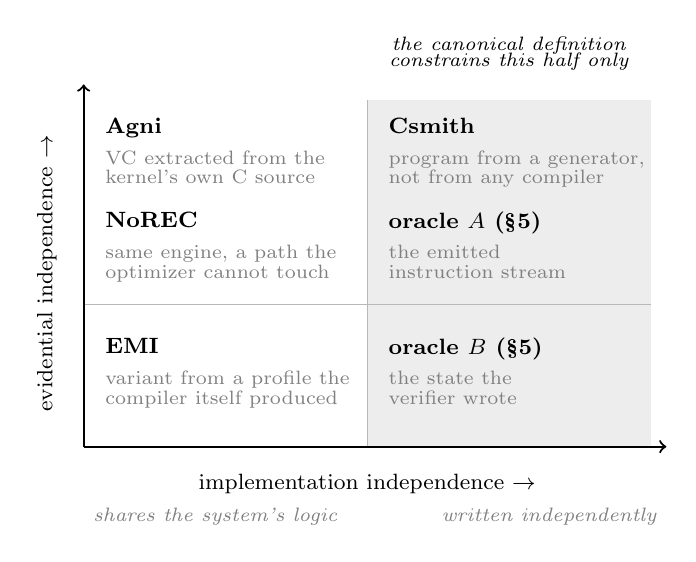
\begin{tikzpicture}[x=1mm,y=1mm,font=\footnotesize]
  \definecolor{gridgrey}{gray}{0.72}
  \definecolor{bandgrey}{gray}{0.93}
  %% Layout (B feedback): a column-filling width (76mm), a height cut in half
  %% (44mm), a font one size larger. Because the top half carries two entries
  %% (Agni, NoREC) it is taller than the bottom; the middle line is semantic, not a ratio.
  \fill[bandgrey] (36,0) rectangle (72,44);
  \draw[gridgrey] (0,18) -- (72,18);
  \draw[gridgrey] (36,0) -- (36,44);
  \draw[->,thick] (0,0) -- (74,0);
  \draw[->,thick] (0,0) -- (0,46);

  \node[anchor=north] at (36,-2.2) {implementation independence $\rightarrow$};
  \node[rotate=90,anchor=south] at (-2.2,22) {evidential independence $\rightarrow$};
  \node[anchor=north west,gray,font=\scriptsize\itshape] at (0,-6.5) {shares the system's logic};
  \node[anchor=north east,gray,font=\scriptsize\itshape] at (74,-6.5) {written independently};

  %% each entry is two nodes: a bold name + a gray two-line description
  \node[anchor=north west] at (1.5,43) {\textbf{Agni}};
  \node[anchor=north west,align=left,font=\scriptsize,text=gray] at (1.5,38.8) {VC extracted from the\\[-1pt]kernel's own C source};
  \node[anchor=north west] at (1.5,31) {\textbf{NoREC}};
  \node[anchor=north west,align=left,font=\scriptsize,text=gray] at (1.5,26.8) {same engine, a path the\\[-1pt]optimizer cannot touch};
  \node[anchor=north west] at (37.5,43) {\textbf{Csmith}};
  \node[anchor=north west,align=left,font=\scriptsize,text=gray] at (37.5,38.8) {program from a generator,\\[-1pt]not from any compiler};
  \node[anchor=north west] at (37.5,31) {\textbf{oracle $A$ (\S5)}};
  \node[anchor=north west,align=left,font=\scriptsize,text=gray] at (37.5,26.8) {the emitted\\[-1pt]instruction stream};
  \node[anchor=north west] at (1.5,15) {\textbf{EMI}};
  \node[anchor=north west,align=left,font=\scriptsize,text=gray] at (1.5,10.8) {variant from a profile the\\[-1pt]compiler itself produced};
  \node[anchor=north west] at (37.5,15) {\textbf{oracle $B$ (\S5)}};
  \node[anchor=north west,align=left,font=\scriptsize,text=gray] at (37.5,10.8) {the state the\\[-1pt]verifier wrote};
  \node[anchor=south,align=center,font=\scriptsize\itshape] at (54,46.5)
    {the canonical definition\\[-2pt]constrains this half only};
\end{tikzpicture}}%
\ifdim\wd0>\columnwidth
  \typeout{FIGWIDTH-ERROR box=\the\wd0 column=\the\columnwidth}%
\fi
\usebox0
\caption{The two axes, with the techniques of Section~7 placed on both. Height is
what an oracle reads: low means it reads what the system produced, high means it reads
something upstream of that. The shaded
half is what a pseudo-oracle is defined to be~\cite{barr2015oracle}: the condition
$f_1 \neq f_2$ fixes a horizontal position and says nothing about height. Agni and
oracle $B$ are mirror images---one encodes the component's own logic but reads its
source, upstream of every value it computes; the other is written independently but
reads what the component produced. Csmith occupies the corner it never claims: its
independence argument is made on the horizontal axis, while what protects it is its
height.}
\label{fig:axes}
\end{figure}


\subsection{The axis is component-relative}

Evidential independence is not a relation between an oracle and a system. It is a
relation between an oracle and the \textbf{component under test}, and an oracle may
share almost all of a system with the code it judges while remaining evidentially
independent of the part it is judging.

NoREC is the clean illustration~\cite{rigger2020norec}. Its reference is the same
database engine: same parser, same storage, same execution. What it changes is that
the query is rewritten into a form the optimizer cannot apply to. Relative to the
optimizer---the component under test---the reference's evidence does not pass
through the code being judged. Relative to the execution engine, it plainly does.

Read component-relatively, the axis predicts the shape of the limitation NoREC's
authors report, and they report it: ``both the unoptimized and optimized query can
yield an incorrect result''. Their framing is that metamorphic testing cannot
establish a ground truth, which is true and coarser. The component-relative reading
says something sharper than ``no ground truth''---it says \emph{which} defects
escape and which do not, and it says so from the construction rather than from
experience.

The same reading places Equivalence Modulo Inputs~\cite{le2014emi}: its variants are
derived from a profile of the program under test, so its evidence passes through the
system for everything except the presence of code that the profile marked
unexecuted. Both techniques are effective. Both are evidentially entangled with some
component of the system they judge. Neither entanglement is an error; what is
missing is a name for it, and therefore a way to say in advance what it costs.

\subsection{What the axis does not explain}

An axis that explained every failure would be a slogan. The case study of Section~5
catalogues six mechanisms by which an oracle can fail to fire on a real defect, each
anchored to a specific fix. Input provenance accounts for two of them: the reference's
ground truth is itself produced by the defective component, and the oracle reads a
field the defect corrupts.

The remaining four are distinct, and none follows from provenance. The deviation may
be conservative---wider than the truth rather than wrong---so it is not a violation
of the property being tested at all. The oracle's predicate may be asymmetric, so
that one direction of disagreement is required to stay silent. The mechanism the
detector uses to create the condition it observes may be unable to create it. Or the
observation may require surviving an event that is fatal by construction.

\subsection{Why practice does not notice}

The failure this axis describes is silent by construction. Evidentially entangled
agreement is indistinguishable, from inside a testing campaign, from genuine
agreement: both look like a clean run. A team learns that its oracle was blind to a
class only when someone else finds a defect of that class by other means, which may
be years later or never.

This is the reason the axis needs a procedure rather than a warning. It cannot be
discovered from one's own results, because the results of an entangled oracle look
exactly like success. It has to be computed---before the oracle is built, from
material the project already has. That procedure is the subject of the next section.


\section{The Procedure}
%% DRAFTED — see paper/procedure.tex.
%% Population independence is a PRECONDITION (3.2), not a caution: violating it
%% yields no bound at all. Cost is foregrounded (3.5): the procedure aims
%% calibration rather than replacing it.
The axis of Section~2 is only useful if it can be applied before the work it is
meant to inform. This section gives the procedure that does so, and its defining
property is cost: it reads source and nothing else. No system is built, nothing is
executed, and no test campaign is run. The output is an upper bound on an oracle's
reach, obtained while the oracle is still a design.

\subsection{Inputs}

The procedure takes two inputs.

The first is the oracle \emph{design} $O$, characterized not by its implementation
but by its \textbf{consumption set}: the artifacts $O$ will read in order to form
its judgement. Naming this set requires no code, which is what makes the procedure
a pre-build one. The set must be named at the granularity of individual artifacts
or fields---``the profile of executed basic blocks'', ``the range fields of the
tracked abstract state''---and not as ``the system's output'', because the answer
differs per artifact. It must also be named relative to the \emph{component} under
test rather than the whole system, for the reason given in Section~2: an oracle may
share most of a system with the code it judges and still be evidentially
independent of the part that matters.

The second is a defect population $P$ drawn from the system under test, and it
carries a precondition.

\subsection{Precondition on the population}

\textbf{$P$ must be drawn independently of any oracle's findings.} A population
assembled from what some tool reported measures the sighted side of that tool and
cannot bound the blind side of any tool, including itself. The natural constructions
that satisfy the precondition are exhaustive over some independently chosen frame:
every fixed defect in a release window, or every fix touching a named component in
the project's history. The natural construction that violates it is the appealing
one---the bug list a technique published---because it is already assembled,
already curated, and already classified.

This is a precondition and not a caution: if $P$ is drawn from a tool's findings,
the procedure does not yield a weaker bound, it yields no bound at all. We state it
formally because it does not transfer on its own. Having applied it correctly to the
system in Section~5---partitioning the historical population by what an oracle
\emph{could} observe, not by what it had found---we nonetheless proposed, when
moving to a second system, to classify the defect list that a published technique
had itself reported. The asymmetry had been learned in one context and did not
survive the move to another, which is the argument for writing the procedure down
rather than treating it as judgement.

A second requirement on $P$ is weaker but must be reported: the criterion selecting
$P$ should not correlate with visibility. A frame such as ``defects whose fix
message quotes internal state'' is convenient and biased, because the property that
makes a defect easy to read may also be the property that made it findable.

\subsection{The step}

For each defect $d \in P$, ask one question:

\begin{quote}
Does $d$ corrupt an artifact in $O$'s consumption set?
\end{quote}

\noindent Three answers are permitted.

\begin{itemize}
\item \textbf{Yes} --- $O$ consumes the corruption and reproduces it. $d$ is in
      $O$'s blind class, structurally and regardless of $O$'s predicate.
\item \textbf{No} --- $d$ corrupts nothing $O$ consumes. This answer covers two
      situations that must be kept apart. If $d$ lies in an artifact $O$ never reads
      at all, $O$ is blind to it as surely as in the first case, for a different
      reason. If $d$ lies in something $O$ does examine, $O$ \emph{may} observe it,
      subject to its predicate covering the class---a necessary condition, not a
      sufficient one. The reproducibility measurement of Section~4.5 found that
      independent readers split exactly on this seam, which is why it is named here.
\item \textbf{Undecided} --- the fix does not settle the question from source.
\end{itemize}

Two disciplines make the step reliable, and both were earned rather than assumed.
First, \emph{decide from the source of the fix, never from its title or summary}.
In an earlier partition of forty fixes, four carried titles that named a
component the diff did not touch; a classification taken from titles would have been
wrong in one case in ten. Second, \emph{Undecided is a bucket, not a default}. A
procedure that silently resolves ambiguity produces a bound it cannot support, and
a count of undecided cases is part of the result rather than an embarrassment in it.

\subsection{Output, and what it is not}

The partition yields $\mathrm{reach}(O) \le |\{d : \text{No}\}| / |P|$, an
\emph{upper} bound, and the slack in it has a name: predicate coverage. A defect the
oracle does not consume may still lie in an arm the oracle never implemented, and
$|\{\text{No}\}|$ counts it anyway. In Section~5 the bound is $1/57$ and the
realized reach is $0/57$; the difference is one such arm. This slack is not
irreducible before a build, because which arms an oracle implements is a property
of the oracle's source, readable the same way the partition is. Being outside the
blind class is necessary for observation and
not sufficient: the oracle's predicate must also cover the class. In Section~5 the
bound is one defect in fifty-seven, and the realized reach is zero, because that one
lies in a part of the predicate the oracle did not implement. A procedure that
promised reach rather than bounding it would have promised one defect and delivered
none on its first application.

\subsection{Why the cost matters}

The procedure's value is not that it is rigorous but that it is cheap enough to run
before committing. Calibrating a single oracle against a single real defect, in the
manner of Section~4, costs a build of the system at the defect and another at its
fix; in our case study that is tens of minutes of machine time per pair and a
configuration that must be held byte-identical across the two. The procedure costs
opening one commit per defect and reading the function it changes.

The asymmetry is the point: run the procedure over the whole population first, then
spend calibration only where it says the oracle should be able to see. The procedure
does not replace calibration---it aims it.


\section{Evaluating a Procedure}
%% DRAFTED — see paper/evaluation.tex.
%% NOT "we ran our tool on a benchmark": there is no tool to score. Four
%% answerable questions of unequal strength (bound held / auditable / changed a
%% decision / generalizes), and a fifth named as unmeasured (reproducibility).
%% 4.1 splits confirmatory from held-out and reports n=1 as n=1.
%% 4.4 reports the absence of external validation as a RESULT, per the fourth
%% contribution — not as an apology.
A procedure is not a tool, and the question ``does it work'' does not reduce to a
benchmark score. What Section~3 produces is a partition and a bound, not a
measurement, so this section states what evaluating such an output can and cannot
mean before Section~5 applies it.

Four questions are answerable, and they are not equally strong. A fifth is not
answerable here and is named as such.

\subsection{Did the bound hold?}

The partition claims that defects corrupting an artifact the oracle consumes are
invisible to it. The claim is testable one defect at a time: build the system at the
defect, run the oracle, and see whether it fires.

The evidence divides, and the division matters. Most calibration in Section~5 was
carried out before the partition existed and for other oracles, so it does not test
this partition. Of the calibration performed afterwards, three pairs were
\emph{selected using} the partition and are therefore confirmatory rather than
independent: the partition said where to look, and looking there succeeded.

Twenty-nine cases are genuinely held out. One was the original: a defect classified as
invisible by the procedure alone---three source lines aligned, no system built---and
checked afterwards against the fix and the oracle's own predicate. Twenty-eight more were
added under a pre-registration discipline, in three batches, and the discipline is the
part worth stating. The frame was fixed by a mechanical query, the sample drawn by a
content-independent rule, and each case classified from the kernel diff alone with a
falsifiable prediction attached. Classifications were committed \emph{before} any
verification ran, in a separate commit from the results, so the ordering is not a
claim about our conduct---it is visible in the artifact's history.

All twenty-eight predictions held, and the composition matters more than the count.
Twenty-one corrupt nothing the oracle consumes, so they answer the step's second
case rather than testing the bound; eighteen of those lie off the
state-equivalence path altogether. Seven tested the blind bound---the fields at issue
were a precision flag, register identities, a pointer type, and stack-slot
metadata, each read from the system's own capture rather than recomputed---and all
seven were confirmed blind.

The first two batches drew from an unfiltered frame and produced no case touching
the predicate at all, leaving the bound's upper arm untested. A third batch was
drawn from a declared stratum---the same frame restricted to fixes whose
\emph{message} mentions pruning or state equivalence---and the stratification is
defensible for a measured reason: in an earlier population, four fixes in forty
carried titles naming a component the diff did not touch, so the message does not
determine the classification the source must still make. That batch supplied the
missing case. A fix replacing the scalar arm's equality test with an
identity-mapping check was classified visible, and the oracle implements exactly
that arm---indeed it is the arm on which the oracle's own calibrated positive
fires. One further case is sharper than either arm: a fix to a second comparison
function, correctly classified as touching the predicate, which the oracle
nonetheless cannot see because it does not model that function. Predicate does not
imply visible, and the held-out set now contains an instance rather than an
assertion.

Two further limits belong here rather than in Section~6, because they bound what
these twenty-eight establish, and the first needs a distinction to be read
correctly. Two separate acts in this study are performed from source. Classifying a
defect from its fix, without building anything, is not a shortcut---it is the
procedure, and doing it any other way would not be testing the procedure at all.
Checking afterwards whether the field that defect touches enters the oracle's
verdict as a consumed value or an independently recomputed one is a different act,
and there a build is stronger evidence than a reading. For twenty-seven of the
twenty-eight, no system was built. For the visible case we built both kernels,
because a reading-only confirmation of the one prediction on the visible side would
have been the weakest link in the study, and what the build returned is more useful
than a confirmation. On the first run the oracle was \emph{silent} on the defective
kernel, although the capture contained exactly the pair the fix's own commit message
describes. The cause was not the predicate: the oracle routes captures to an
era-specific implementation of the comparison by their print format, the 2023 format
is shared with a 2021 era whose comparison legitimately had no identity check, and
the oracle had no arm for the year in between. The source-level reading ``the arm is
implemented'' had been true of one path through the oracle and false of the path this
input took. With the era stated explicitly the oracle fired on the defective kernel
with the predicted arm and was silent on the fixed one, where the pruning event
itself no longer occurs; the same capture under the old routing stays silent. We
count this as a built calibration pair, not as a held-out confirmation, because the
oracle was changed after the first run; and we count the first run as the study's
sharpest result, because it is the axis observed inside the oracle: what the oracle
did was decided by what it read. None of this changes the count. The blind side of
the bound rests on seven held-out cases; the visible side rests on one, drawn from a
stratified batch. The build hardens that one case; it does not add a second, and the
asymmetry is permanent in this study.

The second limit is a wording error of ours. One prediction's falsification
condition, as written in the first batch, conflated ``modelled in the oracle'' with
``independently recomputed by the oracle''; the substantive criterion is the second,
the wording said the first, and a stricter reading would score that case ambiguous
rather than confirmed. The condition was corrected before the second batch, and both
readings are recorded.

\subsection{Can a reader check it?}

For a procedure whose output is a classification, auditability is a more appropriate
evaluation than accuracy, and a stronger one to offer. Every decision in the
partition cites the fix that anchors it and the location in that fix which settles
the question. The unit of verification is one commit: a reader who doubts a row can
open it and re-derive the decision in minutes, without the system, the corpus, or
any part of our infrastructure.

This is what a classification procedure can offer in place of a score. The claim is
not ``trust the partition'' but ``check any row of it''---and it now holds for every partition
in the paper. It did not always. The first flagship partition, of forty fixes, was
classified with anchors recorded in an engineering log but without retaining the
per-commit list as one artifact; when a reviewer asked whether its rows could be
checked, they could not be enumerated, and the partition was rebuilt from a
mechanical frame with both raters' files kept (Section~5.3). The lesson is procedural
and we state it as one: a partition's value as evidence depends on keeping the list,
and the cost of not keeping it was a headline number that had to be withdrawn.

\subsection{Did it change what was done?}

A bound that changes no decision has no value regardless of its correctness, and
the strongest evidence that this one does is that two oracles in this project were
built \emph{without} it and paid for that. Oracle $B$ was designed as an independent
reimplementation of the state-equivalence predicate---independent in the only sense
then in use---and its evidential entanglement was discovered afterwards, by reading
the first partition, at which point close to half of the population it had been built
to catch turned out to have been unreachable from the day it was written. A store-location channel in
the same project judged runtime writes against the verifier's own printed claim of
where each store would land; nine successive false findings were traced, one by one,
to that consumed claim rather than to any predicate, and the verdict had to be moved
to an input the verifier did not produce. With the axis in hand neither design would
have been chosen as it was. Both are recorded in the engineering log as discoveries,
which is the point: they were not obvious at the time.

A smaller instance is recorded as well. Before the partition, the next calibration target had been
chosen by reading fix summaries. The partition classified that target as
structurally invisible to the oracle in question and redirected the choice to a
different defect. The redirected target produced a positive calibration; the
original would have required building two versions of the system to discover that it
could not have fired. The procedure replaced a build with a reading.

\subsection{Does it generalize?}

It is not shown here, and the reason is itself a result rather than an omission.
Validating the bound outside one system requires a defect population classified by
whether an oracle could have observed each defect. No such data exists: published
taxonomies organize defects by symptom and by configuration; a technique's own bug
list measures its sighted side and cannot bound anyone's blind one---including its
own; and the scope statements techniques do publish are component-scoped rather than
input-scoped, which Section~7 shows is not the same partition. Section~7 names the study that would supply the missing data and the design
it must have.

\subsection{Reproducibility, measured once}

Two analysts applying Section~3 to the same population should produce the same
partition. We measured this on the twenty-eight held-out cases with a second rater
that had no access to the first rater's labels: an independent model instance given
only the question of Section~3.3, a factual description of the oracle's consumption
set, and the diffs. It is not a human rater, and what the experiment measures is
correspondingly narrower---whether an independent reader of the same source, asked
the same question, gives the same answer.

On the held-out cases, raw agreement was 25 of 28 and Cohen's $\kappa = 0.71$,
substantial but not near-perfect. On the rebuilt flagship partition of fifty-seven,
agreement was 53 of 57 and $\kappa = 0.86$. Both are above the threshold we
pre-registered as falsifying the auditability claim. The second measurement carries a
caveat the first does not: the first rater read the fifty-seven diffs as truncated
excerpts and the second read them in full, and two of the four disagreements are
plainly the first rater's under-reading. Two details matter more than the coefficient. On the held-out cases the second rater
answered \emph{Undecided} twice; the first rater answered it zero times in the
sixty-eight classifications up to that point, which Section~6 had already flagged as
suspicious, and the flag now has a measurement behind it. On the rebuilt flagship
partition each rater answered it once, on different cases. And the three disagreements are not
scattered: all three are fixes that write a \emph{stack slot}, which this oracle does
not consume at all. The first rater called them blind-by-corruption (Yes); the second
called them not-consumed (No) or Undecided. Both readers agree the oracle is blind to
them; they disagree on which of the step's answers that blindness belongs to, and the
step's wording is what is at fault: its ``No'' covers both a defect the oracle could
in principle observe and a defect in an artifact the oracle never reads, and only the
first is potentially visible. Section~3.3 is corrected accordingly. This is also the
right way to read what the model rater delivered and what it did not. The coefficient
does not rescue auditability; it makes auditability measurable. What the experiment
actually produced is the seam, and that finding does not depend on the rater being
human, because the defect it exposed is in the step's wording, not in any reader of
it. A human study would supply an effect size for the corrected step; it would not
supply the correction, which is already in hand.


\section{Case Study}
%% *** HARD CAP: 2.5 PAGES — see the note at the top of this file. ***
%% DRAFTED — see paper/casestudy.tex. Contract honoured:
%%   5.1 the two oracles contrasted at their INPUT (signatures carry it)
%%   5.2 calibration, two anchors per oracle, one of them a required SILENCE
%%   5.3 the procedure applied ahead of the oracle; bound 1/57, realized 0/57 (rebuilt partition; the original 40 was unrecoverable)
%%   5.4 the verification of 2.4 — agreement at volume, for the wrong reason
%% No chronology: nothing here is justified by the order in which it happened.
The subject is the in-kernel eBPF verifier: an abstract interpreter that must prove
memory safety of untrusted programs before the kernel will run them. Two oracles
were built for it, judging different components of the analysis, and everything
about them was held constant except the one thing this paper is about.

Two things happen in this section and they carry different weight. Sections~5.1
and~5.2 \emph{illustrate}: that an oracle reading corrupted state is blind to the
corruption is close to analytic, and no reader should take the calibration pairs as
tests of the axis. The tests are elsewhere---in the partition of Section~5.3, whose
composition is an empirical fact about this population and could have come out
otherwise; in the held-out predictions of Section~4.1; and in Section~5.4, whose
mechanism was not derivable from the definition and had to be run to be found.

\subsection{Two oracles, one difference}

Oracle~$A$ judges the verifier's \emph{liveness analysis}---the analysis deciding
which registers must be compared when two abstract states meet. Oracle~$B$ judges
the verifier's \emph{state-subsumption predicate}---the decision that one abstract
state is covered by another, which authorizes pruning the search.

Both are independent reimplementations, written from the algorithm rather than from
the code, sharing no source with the component they judge. Both follow the same
rule: where the model cannot decide, it refuses and the case is counted, rather than
approximated. Both were exercised on the same generated corpus and calibrated by the
same protocol.

The difference is the consumption set, and it is visible without reading either
implementation:

\begin{center}
\ttfamily\footnotesize\raggedright
\begin{tabular}{@{}l@{}}
A: run(const insn *ins, int n, result *out)\\
B: compare(const char *log, cmp *out)
\end{tabular}
\end{center}

\noindent$A$'s premises are the instruction stream---upstream of the component it
judges, and untouched by it. $B$'s premises are the abstract state the verifier
itself wrote. Section~2's axis predicts, from these signatures alone, that $A$
survives defects that corrupt verifier state and $B$ reproduces them.

\subsection{Calibration}

Calibration here means: build the system at a real defect and at its fix, with
configurations held byte-identical, and require the oracle to fire on one and be
silent on the other. Sixteen pairs anchor the map, and ten were established that
way; for the rest the defective state was already printed in the fix's own message,
or the question was decidable by aligning source lines. Appendix~B separates the
three. Two pairs per oracle carry the argument here.

$A$, positive. A defect in control-flow graph construction dropped an edge, so a
register that was live was recorded dead. The oracle reported a single cell---the
instruction and register the fix itself names---on the defective build, and nothing
on the fixed one.

$A$, boundary. A defect made the kernel treat a register as used when it need not
be. The deviation is conservative, and the oracle is \emph{required} to stay silent;
it does. A calibration whose correct outcome is silence is what separates an oracle
from a difference detector.

$B$, positive. A defect in the identity-matching arm of the subsumption predicate.
The oracle fires on the defective build; on the fixed build the objected-to pruning
event does not merely become acceptable, it stops occurring, because the predicate
now refuses the pair.

$B$, boundary, and it is the axis made concrete. A defect corrupts the precision
flag that the predicate reads to decide whether to compare at all. The defective
kernel short-circuits on the corrupted flag; the oracle reads the same flag from the
same state and short-circuits identically. Three lines---the kernel's, that era's
kernel, and the model's---align on the same condition. The classification was
derived from source and required no build.

$B$ is not less careful than $A$. It is blind for a reason legible in its signature.

\subsection{The procedure, applied ahead of the oracle}

The population is fifty-seven fixes to the component's history, and how it was
assembled matters. A first partition of forty fixes was made early in the project and
its per-commit list was not retained; its aggregate---23 blind, 2 predicate, 15
outside---was the paper's headline until the list was found unrecoverable, at which
point the partition was rebuilt under a pre-registered protocol with a mechanical
frame: every fix with a \texttt{Fixes:} trailer touching the state-equivalence files
whose message matches a fixed pattern for printed verifier state, minus the sixteen
calibration pairs and the twenty-eight held-out cases already classified. The frame,
both raters' files, and every anchor are artifacts; Section~4.2's claim now holds for
this partition without qualification. The population satisfies Section~3.2's
precondition: it is not drawn from what any oracle here reported. It does
\emph{not} satisfy the weaker second requirement---the frame selects on printed
internal state, a property that may correlate with how a defect was found---and that
bias is carried into Section~6 rather than left here.

Each fix was classified by the single question of Section~3.3, decided from the
diff, by two raters who did not see each other's labels:

\begin{itemize}
\item \textbf{24 of 57} corrupt an artifact $B$ consumes. Structurally blind.
\item \textbf{1 of 57} changes the predicate itself, in the pointer arm.
\item \textbf{31 of 57} corrupt nothing $B$ consumes. The convenient reading of
this bucket---``outside the state-equivalence path''---is wrong, and the held-out
work of Section~4.1 supplied the counterexample: a fix that adds a guard
\emph{in front of} the call to the comparison, changing neither the comparison nor
any field $B$ reads, yet sitting in the middle of the path. The bucket is defined by
the consumption set, exactly as Section~3.3 asks, and it mixes defects that are off
the path with defects that are on it in a part no oracle here models.
\item \textbf{1 of 57} undecided from source.
\end{itemize}

The bound is therefore $\mathrm{reach}(B) \le 1/57$. The realized reach is $0/57$:
the one predicate defect lies in the pointer arm, which $B$ does not implement---the
gap between a necessary condition and a sufficient one that Section~3.4 insists on.
The second rater's partition differs in four rows and puts the blind share at 47\%
rather than 42\%; two of the four are cases where the first rater read a truncated
excerpt and the second read the full diff, so the truth is likely between them.

Read the other way: within this frame the more sophisticated of the two oracles is
structurally blind to \textbf{42\%} of the defects and can target \textbf{2\%}. Both
numbers are properties of the frame as much as of the oracle---Section~6 measures the
frame's enrichment for the oracle's own path at about threefold, and on the
unfiltered complement the on-path share is 3 of 20 with no predicate defect among
them---and both were obtainable before the oracle existed, from material the project
already had, at the cost of opening fifty-seven commits.

\subsection{What the campaign could not have told us}

Section~2.4 argued that this failure is silent by construction. The case study
supplies the instance.

Across every run these oracles performed, agreement was total. The blind class is
not a region where an oracle disagreed and the disagreement was misread; it is a
region where it agreed, at volume, for the wrong reason. Nothing in the campaign's
own output distinguishes that agreement from the sound kind. The blindness became
visible only when the question was put to an external population of real
defects---which is the procedure, and is why it is a procedure and not a caution.
Table~\ref{tab:map} reduces the resulting map to the rows this section argues from;
Appendix~A carries all 56 cells.

The same dependence bounds what an entangled oracle can find when it does fire, and
the system under test makes the mechanism legible. A third channel in this subject
reads the verifier's own internal assertion: the kernel checks its register
invariants and reports a violation as its own bug. That reference is the component's
account of itself, and it carries the component's judgement about which states are
worth asserting over---including the recovery attached to that judgement. Detection
and repair are the same function here: the check reports the violation and, unless a
test flag makes it fatal, widens the offending register and continues, at five call
sites none of which is a memory access. Every defect this channel can report is
therefore one at a point the authors anticipated well enough to install a fallback.
When the channel did finally disagree with the kernel---on a state the verifier's own
invariant forbids, reproducing on the current tip and attributable to a single
commit---a controlled experiment put the emptied register into a memory access and
found the consequence was refusal, not unsoundness. The agreement was uninformative
and the disagreement was inconsequential for one reason: what the oracle reads is
what the component already says about itself.

A run-verified refinement sharpens what ``reads'' means here, and it is not the same
claim as component-relativity. The boundary pair of Section~5.2 was read there as
shared evidence: the oracle consumes the corrupted flag and short-circuits with the
kernel. Running it establishes something narrower. A consumed value need not merely
feed the oracle's own recomputation; it can decide whether that recomputation happens.
The comparison this oracle reimplements begins, in the component, with a short-circuit
on that same bookkeeping flag---a register never marked precise is accepted without
examination---and any faithful model must mirror it, so the flag the component wrote
governs the model's independent arithmetic as a switch rather than as an operand. Fed a capture in which
a register's range had been emptied by an upstream defect, the oracle's range
comparison never executed: every scalar register was short-circuited out and the
oracle agreed without looking. The switch is therefore what makes that pair a boundary, and the
measurement says so rather than inferring it. This cuts slightly against the
paper's own economy: the bound came from reading, but the mechanism behind one of its
boundaries came from running, and we do not think the mechanism was recoverable
without the run. The procedure bounds; calibration explains. The two are not the same
act and the paper should not be read as claiming the first replaces the second. A defect above
such a switch is not mis-decided; it is never examined---which is a stronger and
narrower statement than blindness by shared value, and the one the axis should be
read to make.

\begin{table}[t]
\caption{Blind-spot map, reduced. \textbullet~calibrated positive;
\textcircled{~}~measured boundary; \rule[0.5ex]{1.6ex}{0.4pt}~structurally blind.
\textbf{An empty cell means untested, not blind}---the distinction the map exists to
preserve. Full matrix with the fix anchoring each cell in Appendix~A.}
\label{tab:map}
\small
\begin{tabular}{lcc}
\toprule
defect class & $A$ liveness & $B$ subsumption \\
\midrule
state, self-inconsistent      &            & \rule[0.5ex]{1.6ex}{0.4pt} \\
state, consistent but wrong   &            & \rule[0.5ex]{1.6ex}{0.4pt} \\
bookkeeping (precision flag)  &            & \textcircled{~} \\
predicate, modelled arm       &            & \textbullet \\
predicate, unmodelled arm     &            & \textcircled{~} \\
liveness / control flow       & \textbullet\ \textcircled{~} & \\
\bottomrule
\end{tabular}
\end{table}


\section{Threats to Validity}
%% DRAFTED — see paper/threats.tex. Each threat names the claim it endangers and
%% what would settle it. The frame-bias one is first because §5.3 already admits
%% it: the population satisfies §3.2's precondition and violates its second,
%% weaker requirement.
Section~4 asked how a procedure can be evaluated at all. This section asks what
could make the specific claims of Section~5 wrong, and what would settle each.

\paragraph{The population's frame is biased, and the direction is now measured.}
Section~3.2 states two requirements on the population. The first---independence from
any oracle's findings---is satisfied. The second is not: the fifty-seven fixes were
selected because their messages quote internal state, which is what makes them
readable. That property may correlate with how a defect was found and reported, so
the frame is not a random sample of the component's defect history.

The held-out work of Section~4.1 measures the bias, because its frame was drawn from
the complement of that filter---fixes in the same component and window whose messages
do \emph{not} quote internal state. In the filtered frame, 25 of 57 defects lie on
the state-equivalence path; in the unfiltered complement, 3 of 20
($p = 0.030$, Fisher's exact, two-sided). Selecting on messages that quote verifier
state over-represents state-equivalence-path defects roughly threefold.

This does not overturn the figures in Section~5.3; it corrects what they are
fractions of. It also exposes an asymmetry between the two requirements of
Section~3.2 that the text there does not anticipate. The first---independence from
findings---was kept, and it protects the bound's logic. The second---a frame not
correlated with visibility---was broken, and it was broken in the direction that
inflates exactly the quantity reported: a frame selected on printed verifier state is
a frame selected on the oracle's own inputs. The two requirements are separable in
principle; in this application the one that failed was the one whose failure flatters
the number. The 42\% blind and 2\% targeted are conditional on a frame enriched
for the very path the oracle operates on, and on an unfiltered frame both shares
fall. What the procedure delivers unconditionally is the classification of a given
population, not a population-independent constant---which is Section~3.4's point,
arriving here as a measurement rather than a caution.

\paragraph{The partition was produced with assistance, and its reproducibility is
measured on the held-out cases only.}
Classification was carried out with automated help, and only the decision-changing
case of the flagship partition was re-derived by hand. Section~4.5 now supplies
inter-rater measurements on both the held-out cases and the rebuilt flagship
partition; the original forty could not be re-rated because its list was not
retained (Section~4.2). Its result cuts both
ways for this threat. Agreement was substantial ($\kappa = 0.71$), so the partition is
not an idiosyncrasy of one reader; but the second rater used \emph{Undecided} where the
first never did, and the disagreements clustered on a seam in the step's own wording.
A human inter-rater study over the full population remains the experiment that would
settle it.

\paragraph{The contrast is two oracles in one system.}
Confounds are held constant rather than randomized: same corpus, same discipline,
same protocol, same author. That is the strength of the design and also its limit.
Two oracles differing in one respect show that the respect matters here; they do not
establish an effect size, and no claim of one is made.

\paragraph{Calibration establishes a channel, not a class.}
Each pair certifies that a specific oracle either fires or cannot fire on one
specific defect. Generalizing from a pair to a class is an inference the pair does
not license on its own, and in this work the generalization is carried by the
partition rather than by the pairs. Where a pair and the partition disagree the pair
wins, since it is the direct measurement.

\paragraph{The subject is one analysis in one system.}
The eBPF verifier is an abstract interpreter whose defects are unusually well
documented, which is why it can serve as a case study at all. That same property
makes it unrepresentative: most systems do not publish the internal state their
defects corrupt, and applying the procedure elsewhere may be harder for reasons this
case study cannot expose.


\section{Related Work}
%% DRAFTED — see paper/related.tex. Contains the pre-registered prediction about
%% EMI that was FALSIFIED, reported as such, plus the confirmed-but-weakly-
%% diagnostic second prediction that is explicitly not counted. Unusual for a
%% related-work section; it is the evidence for the fourth contribution.
\paragraph{The canonical formalism, and where the axis is missing from it.}
The standard survey of test oracles defines a pseudo-oracle as ``an alternative
version of the program produced independently, e.g. by a different programming team
or written in an entirely different programming language''~\cite{barr2015oracle}, and
formalizes it as a pair of executions $f_1(x)\,o_1\;f_2(x)\,o_2$ accepted when
$f_1 \neq f_2 \wedge o_1 = o_2$. The independence condition quantifies over the
implementations $f$; the input $x$ is shared and goes unexamined, as it does in the
survey's own prose---``the output of independently implemented components of the SUT
on the same input value.'' That is the axis's absence stated in one line, in the
definition rather than in an omission: independence is a predicate on the programs,
never on what they read.

\paragraph{Oracle-source taxonomies.}
More recent surveys grade independence, and grade it along the same axis: an
independently developed reference ranks above a comparison among existing
implementations, which ranks above consensus among implementations drawn from a
common origin~\cite{oraclesurvey2026}. Input provenance is not among the axes. The
closest such work comes is a remark on oracles derived from the code itself---that
they accept what the code currently does---which is the coarsest case of the
phenomenon and is not developed into a dimension.

\paragraph{Csmith, and an independence it does not name.}
Csmith generates C programs and compares the outputs of several
compilers~\cite{yang2011csmith}. It states the shared-defect limitation plainly---%
``if that did happen we would not detect that problem; this is an inherent limitation
of differential testing without an oracle''---and then argues that it does not happen,
empirically and over implementations: ``despite the fact that Knight and Leveson found
a substantial number of correlated errors in an experiment on N-version programming,
Csmith has yielded no evidence of correlated failures among unrelated C compilers.''
The argument is about how independently the compilers were built, and it is a good
argument. Read through Section~2, a second reason is available and the paper does not
give it: the program under test is produced by Csmith, that is, by \emph{neither}
compiler, so the evidence never passes through a system under test. The technique sits
on the favourable side of the input axis by construction. This is not a confusion on
its authors' part---the axis had no name to reach for---but it is the sharpest
available demonstration that the property is real and load-bearing before it is
articulated.

\paragraph{NoREC.}
NoREC constructs its reference by rewriting a query into a form the optimizer cannot
apply to, and evaluating it on the same engine~\cite{rigger2020norec}. Read through
Section~2.2, it is the axis realized: evidential independence from the component under
test, purchased by construction, while sharing everything else. Its authors state the
corresponding limitation---``both the unoptimized and optimized query can yield an
incorrect result''---and attribute it to metamorphic testing's inability to establish
ground truth. That attribution is correct and coarser than the component-relative
reading, which says not merely that ground truth is absent but which defects escape
and which do not.

\paragraph{The same subject, a different reference.}
Our case study's component has been verified before. Agni checks the soundness of the
verifier's range analysis by generating verification conditions ``directly from the
Linux kernel's C source code'' and discharging them against an independent soundness
specification~\cite{vishwanathan2023agni}. Placed on the axis, it is the opposite
corner from oracle $B$ of Section~5: its input is the component's source text, which
is upstream of every value the component computes, so no defect in the analysis can
reach it as evidence. What it inherits instead is the faithfulness of the extraction,
which its authors name as a trusted computing base. Two oracles for one component,
sharing a subject and almost nothing else, is what the axis is for; they are the
opposing corners of Figure~\ref{fig:axes}.

\paragraph{EMI, and a prediction we registered and lost.}
EMI derives variants by profiling a program and pruning code the profile marks
unexecuted~\cite{le2014emi}, so its evidence passes through the system under test for
everything except the presence of that code. Before reading the paper we recorded a
falsifiable prediction: that its stated limitations would include the class the axis
implies---defects affecting a program and its variant identically. They do not. The
paper's stated limitations concern extension to other languages, floating-point
equivalence, and undefined behaviour. By the criterion we fixed in advance, the
prediction failed.

A second prediction, that the reported defects would concentrate in components
sensitive to surrounding code, holds---``most of the bugs that Orion found in GCC are
optimizer bugs''---but we do not count it. EMI targets optimizations by construction,
so the observation does not separate our axis from the technique's own stated aim, and
a weakly diagnostic confirmation does not offset a falsified prediction.

\paragraph{What the record does and does not supply.}
Authors do sometimes state what their oracle cannot see: Csmith names the shared-defect
case, and Agni's caveats name the unseen class outright---``Only Range Analysis is
Considered\ldots\ There are other static analyses in the kernel verifier beyond range
analysis.'' The claim that survives contact with these papers is narrower and, for our
purposes, sharper. Where a scope is stated it is stated \emph{by component}: which part
of the system was analysed. It is not stated by what the oracle reads, and the reported
defect taxonomies are organized by symptom---wrong code, crash, performance---and by
configuration, never by whether an oracle could have observed the defect. A
component-scoped caveat cannot be turned into the partition of Section~3, because two
oracles covering the same component can differ entirely in what they consume. That is
why the published record cannot validate this axis, and it is the observation
Section~3 turns into a call---reached by trying and failing rather than by assuming.
We are explicit about what the failed prediction does and does not establish. It
measures the record: what a technique's authors chose to state. It does not measure
the axis, and a reader who took it as validation would be right to object; the
axis's tests are the held-out predictions of Section~4.1, and the failed prediction
is evidence only for the fourth contribution, that the data the procedure needs is
not being collected.

\paragraph{Metamorphic testing and differential testing generally.}
The axis is orthogonal to the choice between a metamorphic relation and a reference
implementation. The survey places metamorphic relations among derived oracles because
``in practice, metamorphic relations are usually manually inferred from a white-box
inspection of a SUT''~\cite{barr2015oracle}---a statement about where the relation
comes from, not about what the check consumes when it runs. Both kinds can be
evidentially entangled, and both can be constructed not to be. What the axis adds is
that the entanglement determines a class rather than a degree, and that the class is
computable in advance.


\section{Conclusion}
%% DRAFTED — see paper/conclusion.tex. Ends on the follow-up STUDY DESIGN, not a
%% gesture: a population drawn independently of any tool, partitioned by oracle
%% visibility. That tests the blind side.
Independence is what makes a differential oracle worth believing, and it is graded
along the wrong axis. Whether the reference was written independently bounds how
much logic it can inherit; what the reference reads bounds which defects it can
inherit, and that is the bound that decides what the oracle will never see. The two
are orthogonal, and only the first has a name.

We named the second, gave a procedure that turns it into a number before the oracle
is built, and applied it once: an oracle built with every care available was
measured, from source alone, to be structurally blind to 42\% of a documented defect
population and able to target 2\% of it---figures conditional on a frame we then
measured to be enriched for the oracle's own path, reproduced by a blind second rater,
and obtainable at the cost of opening fifty-seven commits. Reading gave the bound; explaining why one of its boundaries holds took a
build, and the paper does not claim the first act does the second's work.

The procedure's limit is also its finding. It cannot be validated beyond one system
today, because no defect population anywhere is organized by whether an oracle could
have observed each defect. Taxonomies record what a defect did, not what could have
caught it. The study that would close this is specific rather than gestural: take a
defect population drawn independently of any tool---one release window's
wrong-code defects in a compiler, say---and partition it by whether an oracle of a
given input provenance could have observed each. That measures the blind side, which
a tool's own findings can never do, and it is the first application of the same
procedure to a system its authors did not build.


\appendix
\section{The Full Blind-Spot Map}
%% DRAFTED — see paper/appendixA.tex. 56 cells, 34 of them empty, and the empty
%% cells are labelled UNTESTED where the reader sees them.
The full map is eight defect classes against seven oracles: 56 cells. A filled cell
names the fix that anchors it. \textbf{An empty cell means untested, not blind}---the
distinction the map exists to preserve, and 35 of the 56 are empty.

\newcommand{\Pos}{\textbullet}
\newcommand{\Bnd}{\textcircled{~}}
\newcommand{\Bld}{\rule[0.5ex]{1.6ex}{0.4pt}}

\begin{table*}[htbp]
\caption{\Pos~calibrated positive \quad \Bnd~measured boundary \quad
\Bld~structurally blind \quad (blank)~untested.
Oracles: $\Omega$~parsed-state invariants; V~\textsc{reg\_invariants} verdict;
R~runtime retval/intent; S~store location; L~liveness gate; B~subsumption model;
P~prune differential.}
\label{tab:fullmap}
\scriptsize
\setlength{\tabcolsep}{4pt}
\begin{tabular}{lccccccc}
\toprule
defect class & $\Omega$ & V & R & S & L & B & P \\
\midrule
value tracking, self-inconsistent & \Pos & & & & \Bld & \Bld & \\
value tracking, consistent but wrong & \Bld & \Bnd & \Bnd & \Pos & & \Bld & \Bnd \\
over-approximation (genuinely wide) & \Bnd & \Bnd & & & & & \\
bookkeeping, precision flag & & & \Bld & & & \Bnd & \\
predicate, scalar arm & \Bld & & & & & \Pos & \Bnd \\
predicate, pointer arm & & & & & & \emph{u} & \\
liveness / CFG (the prune's gate) & & & & & \Pos\,\Bnd & & \\
dead-code rewrite (accept $\to$ hang/crash) & \Bld & & \Bnd & \Bnd & & & \\
\bottomrule
\end{tabular}
\end{table*}

\noindent\emph{u}: the arm exists in the component and is modelled by no oracle here;
at least one historical defect lives in it (\texttt{1ad2f5838d34}, 2017). It is a
named gap, not a measured boundary.

\paragraph{Anchors, by cell.} Rows are numbered as in Table~\ref{tab:fullmap}.

\begin{itemize}\setlength{\itemsep}{1pt}\sloppy\emergencystretch=2em
\item[1.] $\Omega$: \texttt{3844d153a41a}, \texttt{049c4e13714e},
  \texttt{ae67b9fb8c4e}, \texttt{3cf2b61eb067} --- four positives.
\item[2.] \texttt{3878ae04e9fc} anchors all five filled cells: positive on S;
  boundary on V (the corrupted registers are never printed), on R (the two kernels
  agree on the returned value), and on P (both sides accept).
\item[3.] \texttt{af9e89d8dd39} on $\Omega$ and V --- the state is consistent and the
  width is real, so both are required to stay silent.
\item[4.] \texttt{f54c7898ed1c} on B: the precision short-circuit of Section~5.4. On
  R the consequence is a hang, and a hang is observable by no oracle here, because
  the VM runner wraps boot in a timeout that cannot tell a hang from a slow round.
\item[5.] B: \texttt{2f2ec8e7730e}, \texttt{fd675184fc7a}, \texttt{cd5b460ed1ec} ---
  three positives on three different arms (identity matching, min/max containment,
  arc containment). P: \texttt{2f2ec8e7730e} is a structural boundary there, because
  the default checkpointing already takes the prune.
\item[7.] \texttt{3157f7e29996} positive, \texttt{871ef8d50e7c} boundary.
\item[8.] \texttt{811c363645b3} on R --- the oracle's own ground truth had been
  rewritten to agree with the defect. \texttt{bc308be380c1} on S --- the verifier
  accepts and the kernel faults while executing, so the observation is fatal by
  construction.
\end{itemize}


\section{Calibration Pairs}
%% DRAFTED — see paper/appendixB.tex. The `evidence' column is the honest part:
%% nine built, five message-quoted, one source-only. It contradicts the loose
%% wording in Sec.1/5.2, which was corrected rather than defended.
One row per pair. \emph{Kind} is what the pair established about the oracle, which is
the reason each was built: a pair that only confirms what was already believed buys
nothing. \emph{Evidence} distinguishes what was measured from what was derived:
\textsc{built}---two kernels compiled from one configuration, differing in the fix
alone, and the oracle run on both; \textsc{quoted}---the defective state read from the
commit message's own printed state, no build; \textsc{source}---a determination made
by aligning source lines, no build and no run.

\begin{table}[h]
\caption{Calibration pairs. P~=~positive (the oracle fired on the defect and was
silent on the fix); B~=~boundary (the oracle was \emph{required} to stay silent, and
did).}
\label{tab:pairs}
\scriptsize
\setlength{\tabcolsep}{2.5pt}
\begin{tabular}{@{}l@{\hspace{4pt}}c@{\hspace{4pt}}c@{\hspace{4pt}}l@{\hspace{4pt}}p{0.46\columnwidth}@{}}
\toprule
fix & oracle & & evidence & what the pair established \\
\midrule
\texttt{3844d153a41a} & $\Omega$ & P & \textsc{quoted} & the oracle was missing the property \\
\texttt{92424801261d} & V & P & \textsc{built} & the state is never printed; another channel was needed \\
\texttt{049c4e13714e} & $\Omega$ & P & \textsc{quoted} & property correct, the log could not be read \\
\texttt{ae67b9fb8c4e} & $\Omega$ & P & \textsc{quoted} & no blind spot; a clean confirmation \\
\texttt{af9e89d8dd39} & $\Omega$,V & B & \textsc{quoted} & the class lies outside this instrument \\
\texttt{811c363645b3} & R & B & \textsc{built} & the oracle's ground truth was rewritten to agree \\
\texttt{3cf2b61eb067} & $\Omega$ & P & \textsc{quoted} & the missing half of an earlier pair's property \\
\texttt{3878ae04e9fc} & S & P & \textsc{built} & the store-location channel, never calibrated before \\
\texttt{3157f7e29996} & L & P & \textsc{built} & the liveness gate's own pair \\
\texttt{871ef8d50e7c} & L & B & \textsc{built} & silence required when the kernel over-approximates \\
\texttt{2f2ec8e7730e} & B & P & \textsc{built} & identity matching; the model's first positive \\
\texttt{bc308be380c1} & S & B & \textsc{built} & verifier accepts, kernel faults; observation is fatal \\
\texttt{fd675184fc7a} & B & P & \textsc{built} & min/max containment---a second, older arm \\
\texttt{cd5b460ed1ec} & B & P & \textsc{built} & arc containment; the input, not the oracle, was the blocker \\
\texttt{f54c7898ed1c} & B & B & \textsc{source} & the precision short-circuit (Section~5.4) \\
\texttt{1ffc85d9298e} & B & P & \textsc{built} & the visible held-out case. Silent on the first run: the oracle selects its era-specific comparison by print format, the 2023 format is shared with a 2021 era whose comparison legitimately had no identity check, and no arm existed for the year between---a routing gap, not a predicate one. Fires with the predicted arm once the era is stated (\S4.1) \\
\bottomrule
\end{tabular}
\end{table}

\noindent Sixteen pairs are listed. Ten were built; five were established from the
state the commit message itself prints; one from source alone. Section~5.2's summary
should be read against Table~\ref{tab:pairs}'s evidence column: the design calls for
two builds per pair, and six of the sixteen did not need them because the defective
state was already on the
record or the alignment was decidable without running anything. Reporting that is
cheaper than pretending otherwise, and it is also the point of Section~3.5---the
procedure aims calibration rather than replacing it, and the cheapest calibration is
the one a commit message has already done.


\bibliographystyle{ACM-Reference-Format}
\bibliography{refs}

\end{document}
